\chapter{动词变位(congugaison)}

\section{直陈式现在时(Indicatif Présent)}

动词总共分为三类:以er结尾,以ir结尾,和以re结尾。
9630个动词以er结尾,597个动词以ir结尾,316个以re结尾。


\subsection{er}
\label{sec:er}


规则变化为:及er变化为对应人称的动词变位结尾:

\begin{table}[H]
  \centering
  \begin{tabular}{p{0.2\columnwidth}p{0.8\columnwidth}}
    \toprule[1.5pt]
    \head{主语(sujet)} & \head{结尾(terminaison)} \\
    \midrule[1.5pt]
    je & -e \\
    tu & -es \\
    il/elle/on & -e \\
    nous & -ons \\
    vous & -ez \\
    ils/elles & -ent \\
    \bottomrule[1.5pt]
  \end{tabular}
  \caption{-er}
\end{table}



比如:
\begin{table}[H]
  \centering
  \begin{tabular}{p{0.2\columnwidth}p{0.8\columnwidth}}
    \toprule[1.5pt]
    \head{主语(sujet)} & \head{动词变位(conjugaison)} \\
    \midrule[1.5pt]
    je & parl\textbf{e} \\
    tu & parl\textbf{es} \\
    il/elle/on & parl\textbf{e} \\
    nous & parl\textbf{ons} \\
    vous & parl\textbf{ez} \\
    ils/elles & parl\textbf{ent} \\
    \bottomrule[1.5pt]
  \end{tabular}
  \caption{parler}
\end{table}

\subsection{ir}
\label{sec:ir}

规则变化为:将ir变化为对应人称的动词变位结尾。

\begin{table}[H]
  \centering
  \begin{tabular}{p{0.2\columnwidth}p{0.8\columnwidth}}
    \toprule[1.5pt]
    \head{sujet} & \head{terminaison} \\
    \midrule[1.5pt]
    je & -is \\
    tu & -is \\
    il/elle/on & -it \\
    nous & -issons \\
    vous & -issez \\
    ils/elles & -issent \\
    \bottomrule[1.5pt]
  \end{tabular}
  \caption{-ir}
\end{table}



\begin{table}[H]
  \centering
  \begin{tabular}{p{0.2\columnwidth}p{0.8\columnwidth}}
    \toprule[1.5pt]
    \head{sujet} & \head{conjugaison} \\
    \midrule[1.5pt]
    je & fin\textbf{is} \\
    tu & fin\textbf{is} \\
    il/elle/on & fin\textbf{it} \\
    nous & fin\textbf{issons} \\
    vous & fin\textbf{issez} \\
    ils/elles & fin\textbf{issent} \\
    \bottomrule[1.5pt]
  \end{tabular}
  \caption{finir}
\end{table}


\subsection{re}
\label{sec:re}


\begin{table}[H]
  \centering
  \begin{tabular}{p{0.2\columnwidth}p{0.8\columnwidth}}
    \toprule[1.5pt]
    \head{sujet} & \head{terminaison} \\
    \midrule[1.5pt]
    je & -s \\
    tu & -s \\
    il/elle/on & -t \\
    nous & -ons \\
    vous & -ez \\
    ils/elles & -ent \\
    \bottomrule[1.5pt]
  \end{tabular}
  \caption{-re}
\end{table}

\begin{table}[H]
  \centering
  \begin{tabular}{p{0.2\columnwidth}p{0.8\columnwidth}}
    \toprule[1.5pt]
    \head{sujet} & \head{conjugaison} \\
    \midrule[1.5pt]
    je & romp\textbf{s}\\
    tu & romp\textbf{s}\\
    il/elle/on & romp\textbf{t} \\
    nous & romp\textbf{ons} \\
    vous & romp\textbf{ez}\\
    ils/elles & romp\textbf{ent} \\
    \bottomrule[1.5pt]
  \end{tabular}
  \caption{rompre}
\end{table}

\section{直陈式复合过去式(Indicatif Passé composé)}

过去时,表示过去发生并完成的动作,这里用composé是因为该时态有助动词+动
词变化(participe passé)组成。

动词中大部分词都用的 avoir,少数用être。反身动词(pronominal vebre)都用être。
动词加直接宾语的,用avoir(pronominal例外)。

规则的变化为:

\begin{table}[H]
  \centering
  \begin{tabular}{p{0.3\columnwidth}p{0.3\columnwidth}}
    \toprule[0.5pt]
    -er & é \\
    -ir & i \\
    -re & u \\
    \bottomrule[0.5pt]
  \end{tabular}
  \caption{regular}
\end{table}


\begin{table}[H]
  \centering
  \begin{tabular}{p{0.3\columnwidth}p{0.3\columnwidth}}
    \toprule[0.5pt]
    -ire & it \\
    -aitre & u \\
    -enir & enu \\
    -endre & ris \\
    \bottomrule[0.5pt]
  \end{tabular}
  \caption{irregular}
\end{table}


\section{直陈式 未完成过去时(Indicatif Imparfait)}

用直陈式现在时第三人称负数(nous)的基部(redical)加上对应的人称变位
后缀:

Les terminisons sont:
\begin{table}[H]
  \centering
  \begin{tabular}{p{0.3\columnwidth}p{0.3\columnwidth}}
    \toprule[1.5pt]
    \keyword{sujet} & \keyword{terminaison} \\
    \midrule[1.5pt]{}
    je & -ais \\
    tu & -ais \\
    il/elle/on & -ait \\
    nous & -ions \\
    vous & -iez \\
    ils/elles & -aient \\
    \bottomrule[1.5pt]{}
  \end{tabular}
  \caption{Les terminaisons de l'imparfait}
\end{table}


\begin{table}[H]
  \centering
  \begin{tabular}{p{0.3\columnwidth}p{0.3\columnwidth}p{0.3\columnwidth}}
    \toprule[1.5pt]
    \keyword{Verbe} & \keyword{Présent} & \keyword{Imparfait} \\
    \midrule[1.5pt]
    aimer & Nous \textbf{aim}ons & J'aim\textbf{ais} \\
    choisir & Nous \textbf{choissi}ons & Tu choissi\textbf{ais} \\
    partir & Nous \textbf{part}ons & Il part\textbf{ait} \\
    pouvoir & Nous \textbf{pouv}ons & Nous pouv\textbf{ions} \\
    fair & Nous \textbf{fai}sons & Vous fais\textbf{iez} \\
    venir & Nous \textbf{ven}ons & Ils ven\textbf{aient} \\
    \bottomrule[1.5pt]
  \end{tabular}
  \caption{Example}
\end{table}


\section{直陈式更早过去式(indicatif plus-que-parfait)}

在passé composé的基础上进行变换,将现在时的助动词变为相应的过去式
(avoir,être的participe),在加上动词的participe。

\begin{itemize}
\item j'étais allé
\item tu étais allé
\item il était allé
\item nous étions allé
\item vous étiez allé
\item ils étaient allé
\end{itemize}



\section{直陈式 简单将来时(Indicatif futur simple)}

规则变化:
\begin{itemize}
\item 在动词原形后面加变位后缀(ai, as, a, ons, ez, ont)
\item 如果以e结尾的,把e去掉后再加后缀
\end{itemize}



\begin{table}[H]
  \centering
  \begin{tabular}{ccc}
    \toprule[1.5pt]
    aimer & boire  \\
    \midrule[1.5pt] 
    j'aimer\keyword{ai} & je boir\keyword{ai} \\ 
    tu aimer\keyword{as}      & tu boir\keyword{as}  \\
    il aimer\keyword{a}      & il boir\keyword{a}  \\
    nous aimer\keyword{ons}     & nous boir\keyword{ons} \\
    vous aimer\keyword{ez}&vous boir\keyword{ez} \\
    ils aimer\keyword{ont}&ils boir\keyword{ont}\\
    \bottomrule[1.5pt]{}
  \end{tabular}
  \caption{indicatif Futur simple}
\end{table}

\section{ 虚拟现在时(subjonctif présent)}

规则变化:

使用第三人称复数的基部(radical)加上动词尾部变化。

\begin{table}[H]
  \centering
  \begin{tabular}{cc}
    \toprule[1.5pt]{} \\
    \keyword{直陈式现在时} & \keyword{虚拟现在时} \\
    \midrule[1.5pt]{}
    je finis & que je finiss\textbf{e} \\
    tu finis & que tu finiss\textbf{es} \\
    il finit & que il finiss\textbf{e} \\
    nous finissons & que nous finiss\textbf{ions} \\
    vous finissez & que vous finiss\textbf{iez} \\
    ils \textbf{finiss}ent & qu'ils finiss\textbf{ent}
  \end{tabular}
  \caption{finir}
\end{table}


如果直陈式现在时的第三人称复数基部和nous,vous的基部不同,则用nous,
vous对应的基部加尾部相应的尾部变化。

\begin{table}[H]
  \centering
  \begin{tabular}{cc}
    \toprule[1.5pt]
    \keyword{直陈式现在时} & \keyword{虚拟现在时} \\
    \midrule[1.5pt]
    je bois & que je \keyword{boiv}e \\
    tu bois & que tu \keyword{boiv}es \\
    il boit & qu'il \keyword{boiv}e \\
    nous \keyword{buv}ons & que nous \keyword{buv}ions \\
    vous \keyword{buv}ez & que vous \keyword{buv}iez \\
    ils \keyword{boiv}ent & qu'ils \keyword{boiv}ent \\
    \bottomrule[1.5pt]
  \end{tabular}
  \caption{boire}
\end{table}




\section{条件式现在时(Conditionnel Présent)}
\label{sec:conditionnel-present}

规则变化:

在indicatif future simple的基部上添加后缀(ais,ais,ait,ions,iez,aient)

\begin{table}[H]
  \centering
  \begin{tabular}{cc}
    \toprule[1.5pt]{}
    \keyword{indicatif future simple} & \keyword{conditionnel présent} \\
    \midrule[1.5pt]{}
    j'irai & j'irais \\
    tu iras & tu irais \\
    il ira & il irait \\
    nous irons & nous irions \\
    vous irez & nous iriez \\
    ils iront & ils iraient \\
    \bottomrule[1.5pt]{}
  \end{tabular}
  \caption{aller}
\end{table}



\section{动词变位助记}

法语中,总共有4大类时态,12小类时态,如图\ref{fig:le-temps}。

\begin{figure}[!ht]
  \centering
  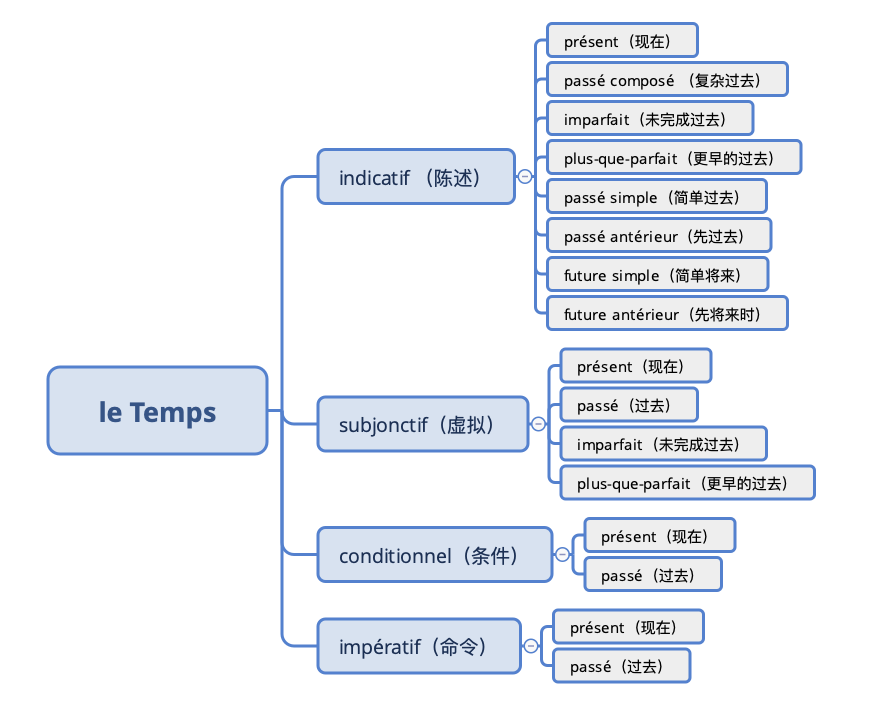
\includegraphics[width=\textwidth]{pic/le-temps}
  \caption{时态}
  \label{fig:le-temps}
\end{figure}


动词变位结尾变化规律如表\ref{tab:congugaison-remember}所示:
\begin{table}[!ht]
  \centering
  \begin{tabular}{p{0.2\textwidth{}}|p{0.2\textwidth{}}|p{0.2\textwidth{}}|p{0.2\textwidth{}}}
    \hline{}
    & \multicolumn{3}{l}{verbe} \\
    \cline{2-4}
    & er & ir & re \\
    \hline
    indicatif présent & e, es, e, ons, ez, ent & is, is, it, issons,
                                                 issez, issent & s, s,
                                                                 t,
                                                                 ons,
                                                                 ez,
                                                                 ent
    \\
    \hline{}
    indicatif passé composé & é & i & u \\
    \hline{}
    indicatif imparfait & \multicolumn{3}{l}{ais, ais, ait, ions, iez,
                          aient} \\
    \hline{}
    indicatif future simple & \multicolumn{3}{l}{ai, as, a, ons, ez,
                              ont} \\
    \hline{}
    subjonctif présent & \multicolumn{3}{l}{e, es, e, ions, eiz, ent}
    \\
    \hline{}
    conditionnel présent & \multicolumn{3}{l}{ais, ais, ait, ions,
                           iez, aient} \\
    \hline{}
  \end{tabular}
  \caption{动词变位助记}
  \label{tab:congugaison-remember}
\end{table}


\begin{itemize}
\item indicatif, inparfait用的présent时态nous的radical
\item indicatif, subjonctif用的présent时态ils的radical
\item conditionnel, présent用的indicatif future simple的radical
\end{itemize}


\begin{itemize}
\item 未完成过去时 用的ai,i,(现在时nous的基)
\item 简单将来时 用的a,ont,(直接加后缀)
\item 虚拟时 用的 e, i (现在时ils的基)
\item 条件时 用的ai, i (将来时的基)
\end{itemize}




%%% Local Variables:
%%% mode: latex
%%% TeX-master: "french"
%%% End:
